\documentclass[landscape,a0paper,fontscale=0.292]{baposter}
%\usepackage[english]{babel}
\usepackage[vlined]{algorithm2e}
\usepackage{times}
\usepackage{calc}
\usepackage{url}
\usepackage{graphicx}
\usepackage{amsmath}
\usepackage{amssymb}
\usepackage{relsize}
\usepackage{multirow}
\usepackage{booktabs}
\usepackage{epstopdf}

\usepackage{graphicx}
\usepackage{multicol}
\usepackage[T1]{fontenc}
\usepackage{ae}
\usepackage{multirow}
\usepackage{rotating}


\graphicspath{{images/}}

\DeclareMathOperator*{\argmax}{arg\,max}
\DeclareMathOperator*{\argmin}{arg\,min}

\newcommand{\x}{\mathbf{x}}
\newcommand{\y}{\mathbf{y}}
\newcommand{\h}{\mathbf{h}}
\newcommand{\w}{\mathbf{w}}

 %%%%%%%%%%%%%%%%%%%%%%%%%%%%%%%%%%%%%%%%%%%%%%%%%%%%%%%%%%%%%%%%%%%%%%%%%%%%%%%%
 %%%% Some math symbols used in the text
 %%%%%%%%%%%%%%%%%%%%%%%%%%%%%%%%%%%%%%%%%%%%%%%%%%%%%%%%%%%%%%%%%%%%%%%%%%%%%%%%
 % Format
 \newcommand{\RotUP}[1]{\begin{sideways}#1\end{sideways}}


 %%%%%%%%%%%%%%%%%%%%%%%%%%%%%%%%%%%%%%%%%%%%%%%%%%%%%%%%%%%%%%%%%%%%%%%%%%%%%%%%
 % Multicol Settings
 %%%%%%%%%%%%%%%%%%%%%%%%%%%%%%%%%%%%%%%%%%%%%%%%%%%%%%%%%%%%%%%%%%%%%%%%%%%%%%%%
 \setlength{\columnsep}{0.7em}
 \setlength{\columnseprule}{0mm}


\definecolor{colorRed}{RGB}{0,50,255}%{120,120,120}


%%%%%%%%%%%%%%%%%%%%%%%%%%%%%%%%%%%%%%%%%%%%%%%%%%%%%%%%%%%%%%%%%%%%%%%%%%%%%
%% Begin of Document
%%%%%%%%%%%%%%%%%%%%%%%%%%%%%%%%%%%%%%%%%%%%%%%%%%%%%%%%%%%%%%%%%%%%%%%%%%%%%
\begin{document}
%%%%%%%%%%%%%%%%%%%%%%%%%%%%%%%%%%%%%%%%%%%%%%%%%%%%%%%%%%%%%%%%%%%%%%%%%%%%%
%% Here starts the poster
%%---------------------------------------------------------------------------
%% Format it to your taste with the options
%%%%%%%%%%%%%%%%%%%%%%%%%%%%%%%%%%%%%%%%%%%%%%%%%%%%%%%%%%%%%%%%%%%%%%%%%%%%%
\begin{poster}{
 % Show grid to help with alignment
 grid=false,
 %Number of columns
 columns=4,
 % Column spacing
 colspacing=0.7em,
 % Color style
 headerColorOne=colorRed,
 borderColor=colorRed,
 % Format of textbox
 textborder=roundedsmall,
 % Format of text header
 headerborder=closed,
 headershape=smallrounded,
 headershade=plain,
 headerheight=0.16\textheight,
 headerFontColor=white,
 boxshade=none,
 background=none,
 bgColorOne=cyan!10!white}
 % Eye Catcher
 { 
    \begin{tabular}{c}
      
\includegraphics{logo/CVPRLogo} \\
    \end{tabular}
 }
 % Title
 {\sc M2CAI Workflow Challenge: Convolutional Neural Networks with Time\\ \vspace{3mm} Smoothing and Hidden Markov Model for Video Frames Classification  \vspace{0.1cm}}
 % Authors
 {Remi Cadene, Thomas RobertNicolas THOME, Matthieu CORD \vspace{0.1cm}\\
 {\small Sorbonne Universit\'{e}s, UPMC Univ Paris 06, LIP6, Paris, France}
 } % University logo
 {
    \begin{tabular}{c}
    %  \includegraphics[height=0.07\textheight]{logo_LIP6} \\ %\vspace{0.1cm} 
      
\includegraphics[height=0.048\textheight]{logo/logos.pdf}  \\
      \\
      \hspace{-10mm}
      
\includegraphics[height=0.075\textheight]{logo/dga.jpg} \hspace{2mm}
      
\includegraphics[height=0.075\textheight]{logo/cnrs} 
    \end{tabular}
    
 }
 

 
 
 
 

%%%%%%%%%%%%%%%%%%%%%%%%%%%%%%%%%%%%%%%%%%%%%%%%%%%%%%%%%%%%%%%%%%%%%%%%%%%%%%
\headerbox{Context}{name=context,column=0,row=0,span=1}{
%%%%%%%%%%%%%%%%%%%%%%%%%%%%%%%%%%%%%%%%%%%%%%%%%%%%%%%%%%%%%%%%%%%%%%%%%%%%%%


\textbf{Goal:} Surgical video frames classification
 
$\triangleright$ Videos of size 1920x1080 Shot at 25 frames per second at IRCAD research center in Strasbourg, France

$\triangleright$ 27 training videos

$\triangleright$ 15 testing videos

$\triangleright$ 8 classes

 \begin{tabular}{cc}
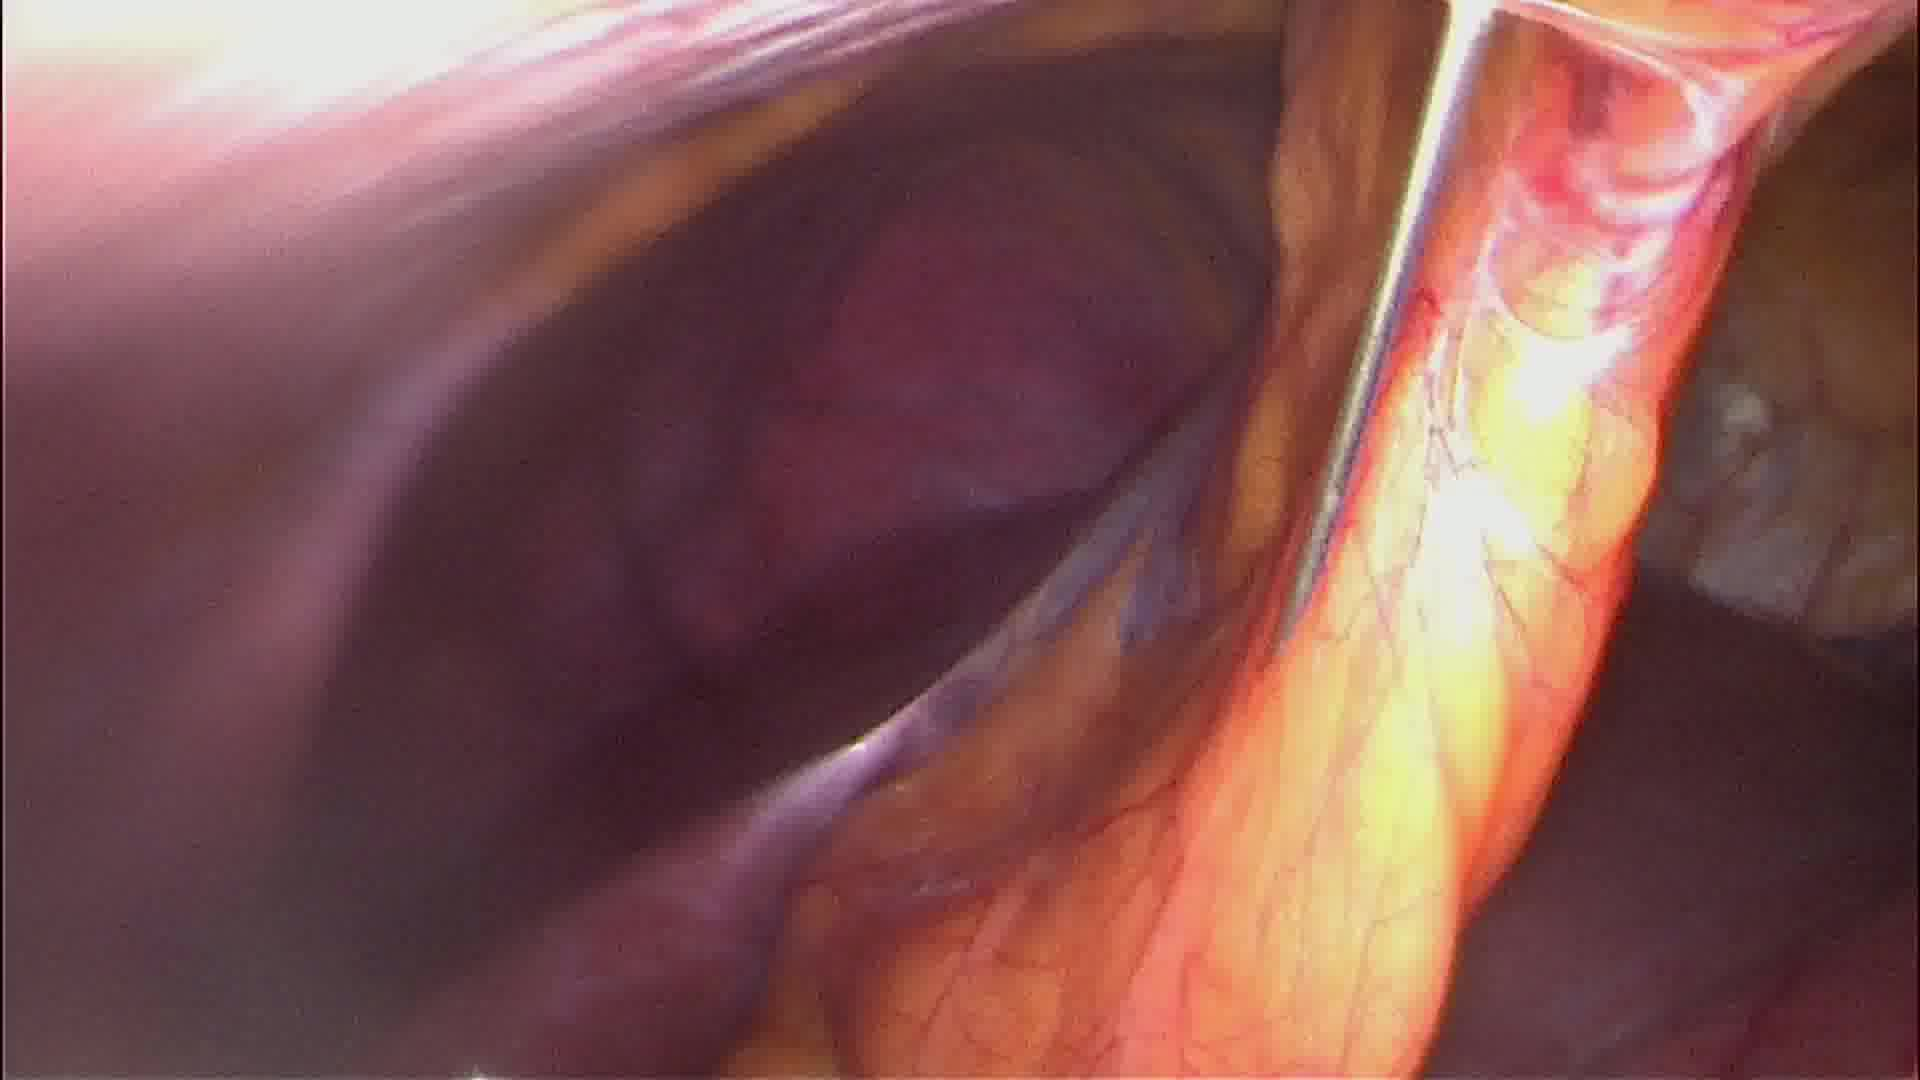
\includegraphics[width=3.5cm]{../slides/images/m2cai.jpg}
& 

\includegraphics[width=3.5cm]{logo/dga.jpg} 
\\
{\em OK for centered object} & {\em KO for ``natural'' image}
\end{tabular}

\vspace{1mm}

$\triangleright$ Online prediction: $P(y | x_i, x_{i-1}, x_{i-2}, ...)$
 
%$\triangleright$ Supervision: full annotations ({\em e.g.} BB) expensive

$\triangleright$ Usefull to
%Weakly Supervised Learning (WSL) framework 

~~ $\triangleright$ Monitor surgeons

~~ $\triangleright$ Trigger automatic actions

%$\triangleright$ End-to-end training 

\vspace{2mm}
\textbf{Our approach (usable in production)}

$\triangleright$ Firstly, we train a classifier using Deep Learning

$\triangleright$ Secondly, we smooth its predictions 

~~ $\triangleright$ Averaging predictions over last 15 frames

~~ $\triangleright$ Then, we use a Hidden Markov Model (HMM) as a "denoizer"

}

% %%%%%%%%%%%%%%%%%%%%%%%%%%%%%%%%%%%%%%%%%%%%%%%%%%%%%%%%%%%%%%%%%%%%%%%%%%%%%%
%   \headerbox{Fully $\rightarrow$ Weakly Deep}{name=model,column=0,below=context}{
% %%%%%%%%%%%%%%%%%%%%%%%%%%%%%%%%%%%%%%%%%%%%%%%%%%%%%%%%%%%%%%%%%%%%%%%%%%%%%%
% 
% $\triangleright$ Standard deep architecture: VGG16
% 
% $\triangleright$ Problem: fixed-size image
% 
% $\triangleright$ Adapt architecture to WSL
% 
% ~~ $\triangleright$ Fully connected layer $\rightarrow$ convolution layer 
% 
% ~~~~~ $\triangleright$ Sliding window approach / shared features
% 
% ~~ $\triangleright$ Spatial aggregation 
% 
% ~~~~~ $\triangleright$ Perform object localization prediction
% 
% 
% }

%%%%%%%%%%%%%%%%%%%%%%%%%%%%%%%%%%%%%%%%%%%%%%%%%%%%%%%%%%%%%%%%%%%%%%%%%%%%%%
  \headerbox{Frames classifier}{name=region,column=0,below=context, above=bottom}{
%%%%%%%%%%%%%%%%%%%%%%%%%%%%%%%%%%%%%%%%%%%%%%%%%%%%%%%%%%%%%%%%%%%%%%%%%%%%%%

\textbf{Creating validation set by random split:}

$\triangleright$ Training set: 22 videos
$\triangleright$ Validation set: 5 videos $\{2,9,10,13,27\}$

\vspace{1mm}

\textbf{Extracting one frame every 25 frames (1 f/s):}

$\triangleright$ Training set: 59,493 images

$\triangleright$ Validation set: 8,062 images

$\triangleright$ Testing set: 28,732 images

\vspace{-2mm}


\textbf{3 approaches using Deep Learning:}

$\triangleright$ Training CNN From Scratch

~~ $\triangleright$ Good: learning representations for this task

~~ $\triangleright$ Bad: maybe not enough data + lot of hyperparameters

$\triangleright$ Pre-trained CNN as Features Extractor + SVM

~~ $\triangleright$ Good: using (good) representations learned on ImageNet 

~~ $\triangleright$ Bad: large semantic gab between ImageNet and this task

$\triangleright$ Fine Tuning a pre-trained CNN 

~~ $\triangleright$ Good: adapting the representations learned on ImageNet for this task

}


%%%%%%%%%%%%%%%%%%%%%%%%%%%%%%%%%%%%%%%%%%%%%%%%%%%%%%%%%%%%%%%%%%%%%%%%%%%%%%
  \headerbox{Deep Learning architecture and methods}{name=reso_results,column=1,row=0,span=2}{
%%%%%%%%%%%%%%%%%%%%%%%%%%%%%%%%%%%%%%%%%%%%%%%%%%%%%%%%%%%%%%%%%%%%%%%%%%%%%%
  
\begin{center}
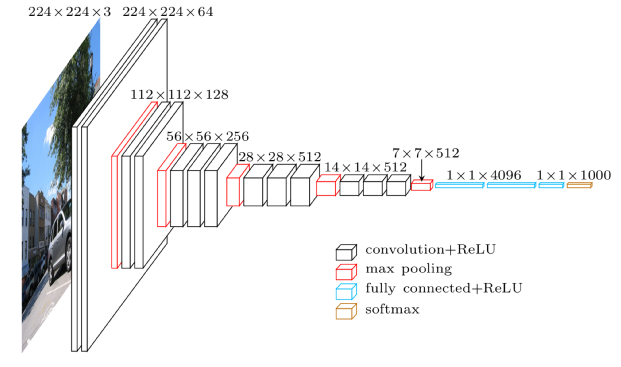
\includegraphics[width=14cm]{../slides/images/vgg16.png}
\end{center}

\vspace{-3mm}
\begin{minipage}[t]{8cm}

$\triangleright$ Fully connected layer $\rightarrow$ convolution layer 

~~ $\triangleright$ Sliding window approach / shared features

\end{minipage} \hfill 
\begin{minipage}[t]{8cm}

$\triangleright$ Spatial aggregation 

~~ $\triangleright$ Object localization prediction

\end{minipage}

}

%%%%%%%%%%%%%%%%%%%%%%%%%%%%%%%%%%%%%%%%%%%%%%%%%%%%%%%%%%%%%%%%%%%%%%%%%%%%%%
  \headerbox{Experiments}{name=lr-cnn,column=1,span=2,below=reso_results,above=bottom}{
%%%%%%%%%%%%%%%%%%%%%%%%%%%%%%%%%%%%%%%%%%%%%%%%%%%%%%%%%%%%%%%%%%%%%%%%%%%%%%

% \begin{center}
% \begin{tabular}{cccccc}
% \hspace{-3.5mm}
%  \includegraphics[height=1.94cm]{000013} & \hspace{-4mm}
%  \includegraphics[height=1.94cm]{003006} & \hspace{-4mm}
%  \includegraphics[height=1.94cm]{2012_004308} & \hspace{-4mm}
%  \includegraphics[height=1.94cm]{COCO_7} & \hspace{-4mm}
%  \includegraphics[height=1.94cm]{15scene} & \hspace{-4mm}
%  \includegraphics[height=1.94cm]{bookstore} \\
%  \hspace{-4mm} VOC 2007 & \hspace{-4mm} VOC 2012 & \hspace{-4mm} VOC12 Action & \hspace{-4mm} COCO & \hspace{-4mm} 15 Scene & \hspace{-4mm} MIT67 
% \end{tabular}
% \end{center}


\begin{minipage}[t]{8cm}

%\vspace{-13mm}

	\begin{center}
		\begin{tabular}{|c|c|c|}
			\hline
			Model & Type & Accuracy (\%) \\
			\hline\hline
			InceptionV3 & Extraction (repres. of ImageNet)& 60.53 \\
			InceptionV3 & From Scratch (repres. of M2CAI) & 69.13 \\
			%InceptionV3 Weldon & 78.18 \\
			InceptionV3 & Fine-tuning (both representations) & 79.06 \\
			\textbf{ResNet200} & \textbf{Fine-tuning (both representations)} & \textbf{79.24} \\
			\hline
		\end{tabular}
	\end{center}

\end{minipage} \hfill 
\begin{minipage}[t]{8cm}

\begin{center}
		\resizebox{300pt}{!}{%
		\begin{tabular}{|c|c|c|c|}
			\hline
			Temporal Method & Accuracy Val (\%) & Jaccard Val & Jaccard Test \\
			\hline\hline
			Avg Smoothing & 85.97 & 74.67 & -- \\
			\textbf{Avg + HMM Online} & \textbf{88.90} & \textbf{81.60} & \textbf{71.9} \\ \hline
			Avg + HMM Offline & 93.47 & 87.59 & -- \\
			\hline
		\end{tabular}}
	\end{center}


{
\scriptsize
[1] Oquab et al. Is object localization for free? {\em CVPR}, 2015.

[2] Durand et al. MANTRA. {\em ICCV}, 2015.

[3] Parizi et al. Automatic discovery of parts. {\em ICLR}, 2015.

[4] Gong et al. Multi-scale orderless pooling. {\em ECCV}, 2014.

}

\end{minipage}


}



%%%%%%%%%%%%%%%%%%%%%%%%%%%%%%%%%%%%%%%%%%%%%%%%%%%%%%%%%%%%%%%%%%%%%%%%%%%%%%
  \headerbox{Hidden Markov Model}{name=learning,column=3,row=0}{
%%%%%%%%%%%%%%%%%%%%%%%%%%%%%%%%%%%%%%%%%%%%%%%%%%%%%%%%%%%%%%%%%%%%%%%%%%%%%%

$\triangleright$ Initial state probabilities

$\triangleright$ Matrix of probabilities of transition between states

$\triangleright$ Gaussian parameters for emissions of observations (mean and co-variance matrix)


%\vspace{2mm}
\begin{tabular}{cc}
\hspace{-3mm} 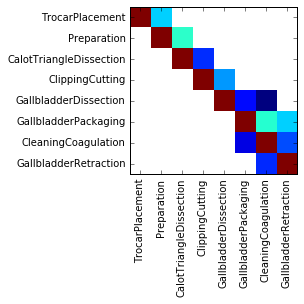
\includegraphics[width=3.9cm]{../slides/images/index.png} & \hspace{-4mm} 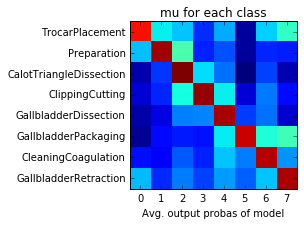
\includegraphics[width=3.9cm]{../slides/images/index2.png} \\
(b) & (c mean) \\
\end{tabular}
%\vspace{-2mm}


%~~ $\triangleright$ Exact and efficient (loss-augmented) inference
}

%%%%%%%%%%%%%%%%%%%%%%%%%%%%%%%%%%%%%%%%%%%%%%%%%%%%%%%%%%%%%%%%%%%%%%%%%%%%%%%
%  \headerbox{Optimizing Ranking Metrics}{name=ranking,column=3,below=learning}{
%%%%%%%%%%%%%%%%%%%%%%%%%%%%%%%%%%%%%%%%%%%%%%%%%%%%%%%%%%%%%%%%%%%%%%%%%%%%%%%
%
%$\triangleright$ Goal: predict a ranking matrix
%
%$\triangleright$ Optimized Average Precision
%
%$\triangleright$ Latent structured output formulation [2]
%
%$\triangleright$ Defined a surrogate upper-bound loss
%
%~~ $\triangleright$ Generalized MANTRA ranking instantiation
%
%~~ $\triangleright$ Exact and efficient (loss-augmented) inference
%
%}


%%%%%%%%%%%%%%%%%%%%%%%%%%%%%%%%%%%%%%%%%%%%%%%%%%%%%%%%%%%%%%%%%%%%%%%%%%%%%%
\headerbox{Visual results}{name=visu,column=3,below=learning}{
%%%%%%%%%%%%%%%%%%%%%%%%%%%%%%%%%%%%%%%%%%%%%%%%%%%%%%%%%%%%%%%%%%%%%%%%%%%%%%

\begin{center}
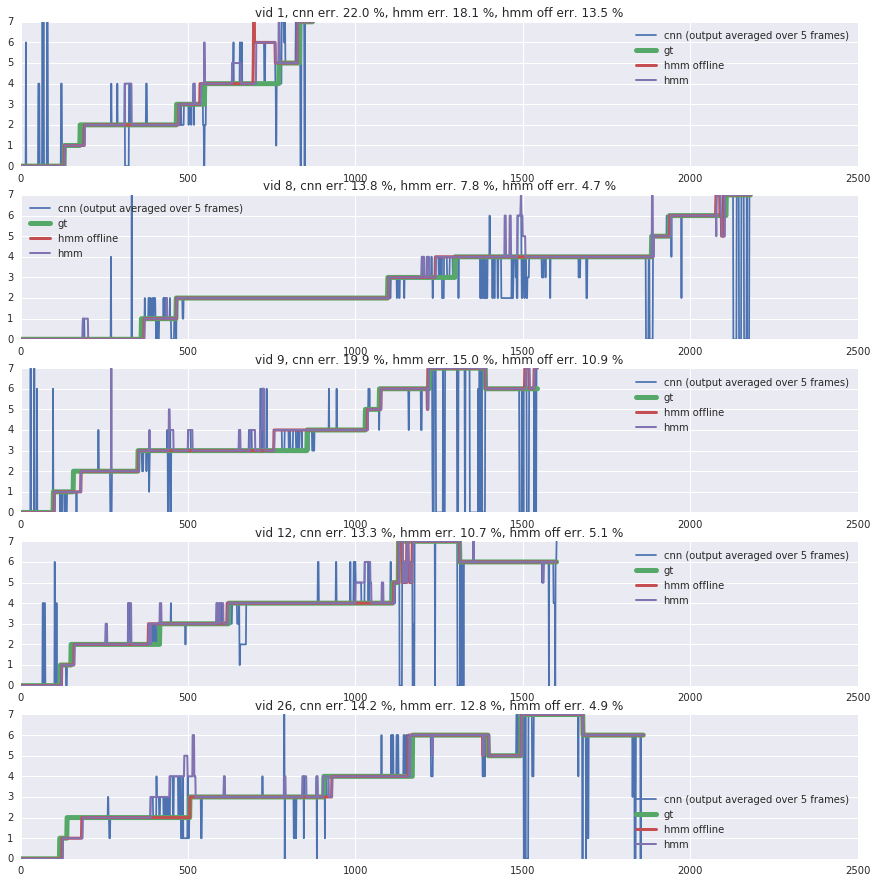
\includegraphics[width=7cm]{../report/images/visu.png}
\end{center}

}

%%%%%%%%%%%%%%%%%%%%%%%%%%%%%%%%%%%%%%%%%%%%%%%%%%%%%%%%%%%%%%%%%%%%%%%%%%%%%%
\headerbox{Conclusion}{name=ouverture,column=3,above=bottom,below=visu}{
%%%%%%%%%%%%%%%%%%%%%%%%%%%%%%%%%%%%%%%%%%%%%%%%%%%%%%%%%%%%%%%%%%%%%%%%%%%%%%

$\triangleright$ Fine Tuning most accurate approach
$\triangleright$ HMM is usefull to smooth the predictions
$\triangleright$ Production ready !

$\triangleright$ Future Work:
~~ $\triangleright$ Fine Tuning CNN on full trainset
~~ $\triangleright$ Ensembling several fine tuned CNNs

}

\end{poster}%
%
\end{document}
